\chapter{TuMag's design and calibration.}

In this chapter we take the first steps of the journey of developing an instrument to observe the Sun. We will define... 

Fabry-Pérot interferometers (FPIs) are widely employed in the field of solar physics. Their spectroscopic and tunability properties make them especially suitable for selecting a narrow spectral band of incoming light. They also offer a two-dimensional view of the solar scene, hence allowing for the implementation of powerful and widespread image post-processing reconstruction techniques, such as phase diversity \citep{PD_etalon} and multi-object multi-frame blind deconvolution (MOMFBD; \citealt{mombfd}), which are difficult to implement in slit-based spectrographs (\citealt{image_spectro}, \citealt{image_spectro_2}). Many state-of-the-art instruments use FPIs as narrowband tunable filters. Among others, these instruments include the spaceborne Polarimetric and Helioseismic Imager \citep[][]{PHI} aboard the Solar Orbiter mission \citep[][]{SO} (SO/PHI); the Imaging Magnetograph Experiment (IMaX) instrument \citep[][]{IMaX}, which flew on the first two flights of the balloon-born SUNRISE observatory (\citealt{SunriseI}, \citealt{SunriseII}); and the Tunable Magnetograph (TuMag) instrument for its third edition. These instruments are based on solid LiNbO$_3$ etalons. Regarding ground-based instruments, some examples include the Crisp Imaging Spectro-Polarimeter (CRISP) at the Swedish 1-m Solar telescope \citep[][]{crisp} at the Observatorio del Roque de los Muchachos in La Palma, Canary Islands; the GREGOR Fabry-Perot Interferometer (GFPI; \citealt{GFPI}, \citealt{GREGOR}) at the Observatorio del Teide in Tenerife, Canary Islands; the Visible Tunable Filter \citep[VTF;][]{VTF} developed for the \textit{Daniel K. Inouye} Solar Telescope \citep[DKIST;][]{DKIST} of the Haleakal\=a Observatory in Hawaii; and the future Tunable Imaging Spectropolarimeter (TIS) of the European Solar Telescope \citep{EST}, all of which are based on air-gapped etalons. 

The SUNRISE III mission aims to study and stablish the relations and couplings between the phenomena ocurring at different layers of the Sun's surface. With this purpose in mind, three different post-focal instruments were included in the design, each of them responsible of observing at different regions of the spectrum. The SUNRISE UV Spectropolarimeter and Imager (SUSI, \textbf{REFERENCIA}), which will observe the spectra between 309 nm and 417 nm; The Sunrise Chromospheric Infrared spectroPolarimeter (SCIP, \textbf{REFERENCIA}), which will observe the near-infrared; and lastly, the Tunable Magnetograph (TuMag), which will observe three spectral lines in the visible, at 525.02 nm, 525.06 nm and 517 nm. 

The design from scratch of an instrument such as this is very complex. There are many things that have to be meticulously designed and tested which span many fields of expertise, like optics, electronics, software, hardware, or thermal design. To avoid undue extension of this thesis, we will focus on the aspects of the design directly related to the optical properties, that is, regarding the spectral, imaging and polarimetric capabilities of the instrument. 

\section{The Tunable magnetograph: TuMag}

The Tunable Magnetograph (TuMag) is a tunable imaging spectropolarimeter designed to deliver high spatial resolution images across multiple spectral lines in four distinct polarization states. Consequently, TuMag is capable of measuring the four Stokes parameters, thus enabling the inference of the three components of the magnetic field and the LOS velocities at all the selected spectral lines. Moreover, this data must be acquired following a series of strict requiremets regarding optical quality, polarimetric efficiencies, required SNR, spectral performance and time limitations. A summary of these requirements is provided in Table \ref{table: Tumags requirements}. 

\begin{table}
    \centering
   \begin{tabular}{cc}
    \hline
    \hline
    Requirements & Value \\
    \hline
    Field of view & $63''$ x $63''$ \\
    RMS wavefront error & $W \sim \lambda / 14$\\
    Spatial sampling & $3 \times 3 $ pixels \\
    Plate scale & $0.0378''$ / pixel \\
    Polarimetric efficiencies & $\epsilon _ {1, 2, 3} \lessapprox \frac{1}{\sqrt{3}}$\\
    SNR ratio & $\left(\frac{S}{N}\right) _ 0 \gtrapprox 1700$ \\
    Spectral resolution & $< 9$ pm\\  
    Spectral lines & Fe I 5250.2 \r{A}, Fe I 5250.6 \r{A} and Mg I $b_2$ 5172.7 \r{A}. \\
    Time for a two-line observation & $< 90$ s\\
    \hline
    \hline
    \end{tabular}
    \caption{Tumag scientific requirements.}
    \label{table: Tumags requirements}
\end{table}

\section{TuMag's design and light path.}

Light is delivered to TuMag by the ISLiD system and subsequently re-imaged onto two cameras where the images are recorded. Before reaching the cameras, the light passes through all the different subsystems of the optical unit. The first components encountered by the light are a blocking prefilter and a the filter wheels. The blocking prefilter, with a wide bandpass centered at 520 nm, is employed to eliminate unwanted spectral ranges. The filter wheels  are comprised by a double-disk system \citep{filter-wheels} that houses the prefilters for selecting specific spectral lines and a series of calibration modules. Specifically, three prefilters are mounted on the second disk of the filter wheel, corresponding to the spectral lines Fe I 5250.2 \r{A}, Fe I 5250.6 \r{A}, and Mg I $b_2$ 5172.7 \r{A}. A detailed overview of the spectral properties of these prefilters will be provided in Section \textcolor{red}{XX}. Additionally, the filter wheel includes a PD plate, which is used to introduce a known defocus into the final image to facilitate image reconstruction techniques, along with a linear polarizer, a plate of micropolarizers, and a pinhole set.

After passing through the filter wheels, the light is directed into the Polarization Modulation Package (PMP), a subsystem derived from the SO/PHI instrument (\citealt{pmp1}, \citealt{PHI}). The PMP's primary function is to modulate the light to produce the different polarization states required to deduce the Stokes components. This is achieved using two liquid crystal variable retarders (LCVRs), which are oriented with their fast axes at 45$^\circ$ relative to each other. These LCVRs induce a retardance on the transmitted light that varies with the voltage applied across the crystals. The system can operate in two distinct modulation schemes: a vector modulation scheme, which generates four independent linear combinations of equally-weighted Stokes components across consecutive observations, allowing for the retrieval of the full Stokes vector after demodulation; and a longitudinal modulation scheme, which generates only two modulations, providing information solely on the intensity and circular polarization.

Following modulation, the light is directed into a LiNbO$_3$ Fabry-Pérot etalon, that likewise IMaX, is in a collimated setup and with a double pass configuration \citep{etalon-doublepass}. In this setup, after traversing the etalon once, the light is redirected by a pair of mirrors to pass through the etalon a second time. This double-pass configuration significantly enhances spectral resolution by narrowing the transmission profile. The LiNbO$_3$ etalon achieves wavelength tuning by varying the refractive index of the cavity through the application of high voltages (ranging from $-4000$ V to $4000$ V) to the mirrors. Compared to air-gapped etalons, these kind of etalons offer the advantage of having no moving parts, which is particularly beneficial for spaceborne or balloon-borne instruments. However, this advantage comes with the need for precautions to prevent discharges caused by air ionization.

The final optical element the light encounters before reaching the cameras is a polarizing beam splitter. At this stage, the light beam is divided into two orthogonal, linearly polarized components, each directed towards a different camera. This dual-beam configuration \citep{lites-doublebeam} is designed to minimize spurious signals induced by jitter of the gondola, as it effectively cancels fluctuations from Stokes I to the other Stokes parameters that may arise due to image motion or solar evolution (\textit{i.e.} cross-talk).

Light then reaches the cameras, where images from both are recorded and stored. After mission recovery, the data is processed on-ground to combine images from the different cameras, modulation states, and spectral lines, ultimately deriving the scientific products. This processing and reduction of the data is accomplished using software specifically developed for TuMag, which will be extensively discussed in Section XX. 

\section{Instrument performance and verification.}

\subsection{Spectral performance.}

TuMag filters wavelengths through a sequential process, beginning with a broad blocking pre-filter that eliminates unwanted portions of the solar spectrum, and followed by a second narrow-band pre-filter that is tuned to the three selected spectral lines. Finally, the LiNbO$_3$ Fabry-Pérot etalon is encharged of selecting a very narrow band around specific wavelengths along the spectral lines. The narrow-band pre-filter and the etalon are critical to TuMag's spectroscopic performance and require careful evaluation during calibration.

The three TuMag pre-filters were custom-manufactured by Materion$^{TM}$ and have a full width at half maximum (FWHM) close to 1 nm. They are centered near the rest wavelength of the three spectral lines at normal incidence, with a peak transmission exceeding 80\% in all cases. Each pre-filter was tuned by adjusting the incidence angle to align the peak transmission wavelength with the spectral line core, a process carried out using a coelostat at the INTA facilities. While this tuning was successful, particularly for the iron lines, the spectral position of the pre-filters was found to be highly sensitive to illumination conditions. This sensitivity was evident from the shifts observed in the pre-filter measurements during the various stages of the assembly process. As illustrated in the left column of Fig.~\ref{fig_tumag: spectroscopic_results}, the variation in the spectral position of the pre-filters is not sufficient to cause the spectral line to be blocked by the pre-filter, but it may result in the spectral line falling on the wing of the pre-filter during observations.

\begin{table}
    \centering
   \begin{tabular}{cc}
    \hline
    \hline
    Property & Value \\
    \hline
    Reflectivity & 0.892 \\
    Thickness & 281 $\mu$m\\
    FWHM (double-pass) & 0.8\\
    Tuning Constant & 3300 V/\r{A}\\
    \hline
    \hline
    \end{tabular}
    \caption{Tumag Fabry-Pérot specifications.}
    \label{table: Tumags etalon}
\end{table}

\begin{figure}
    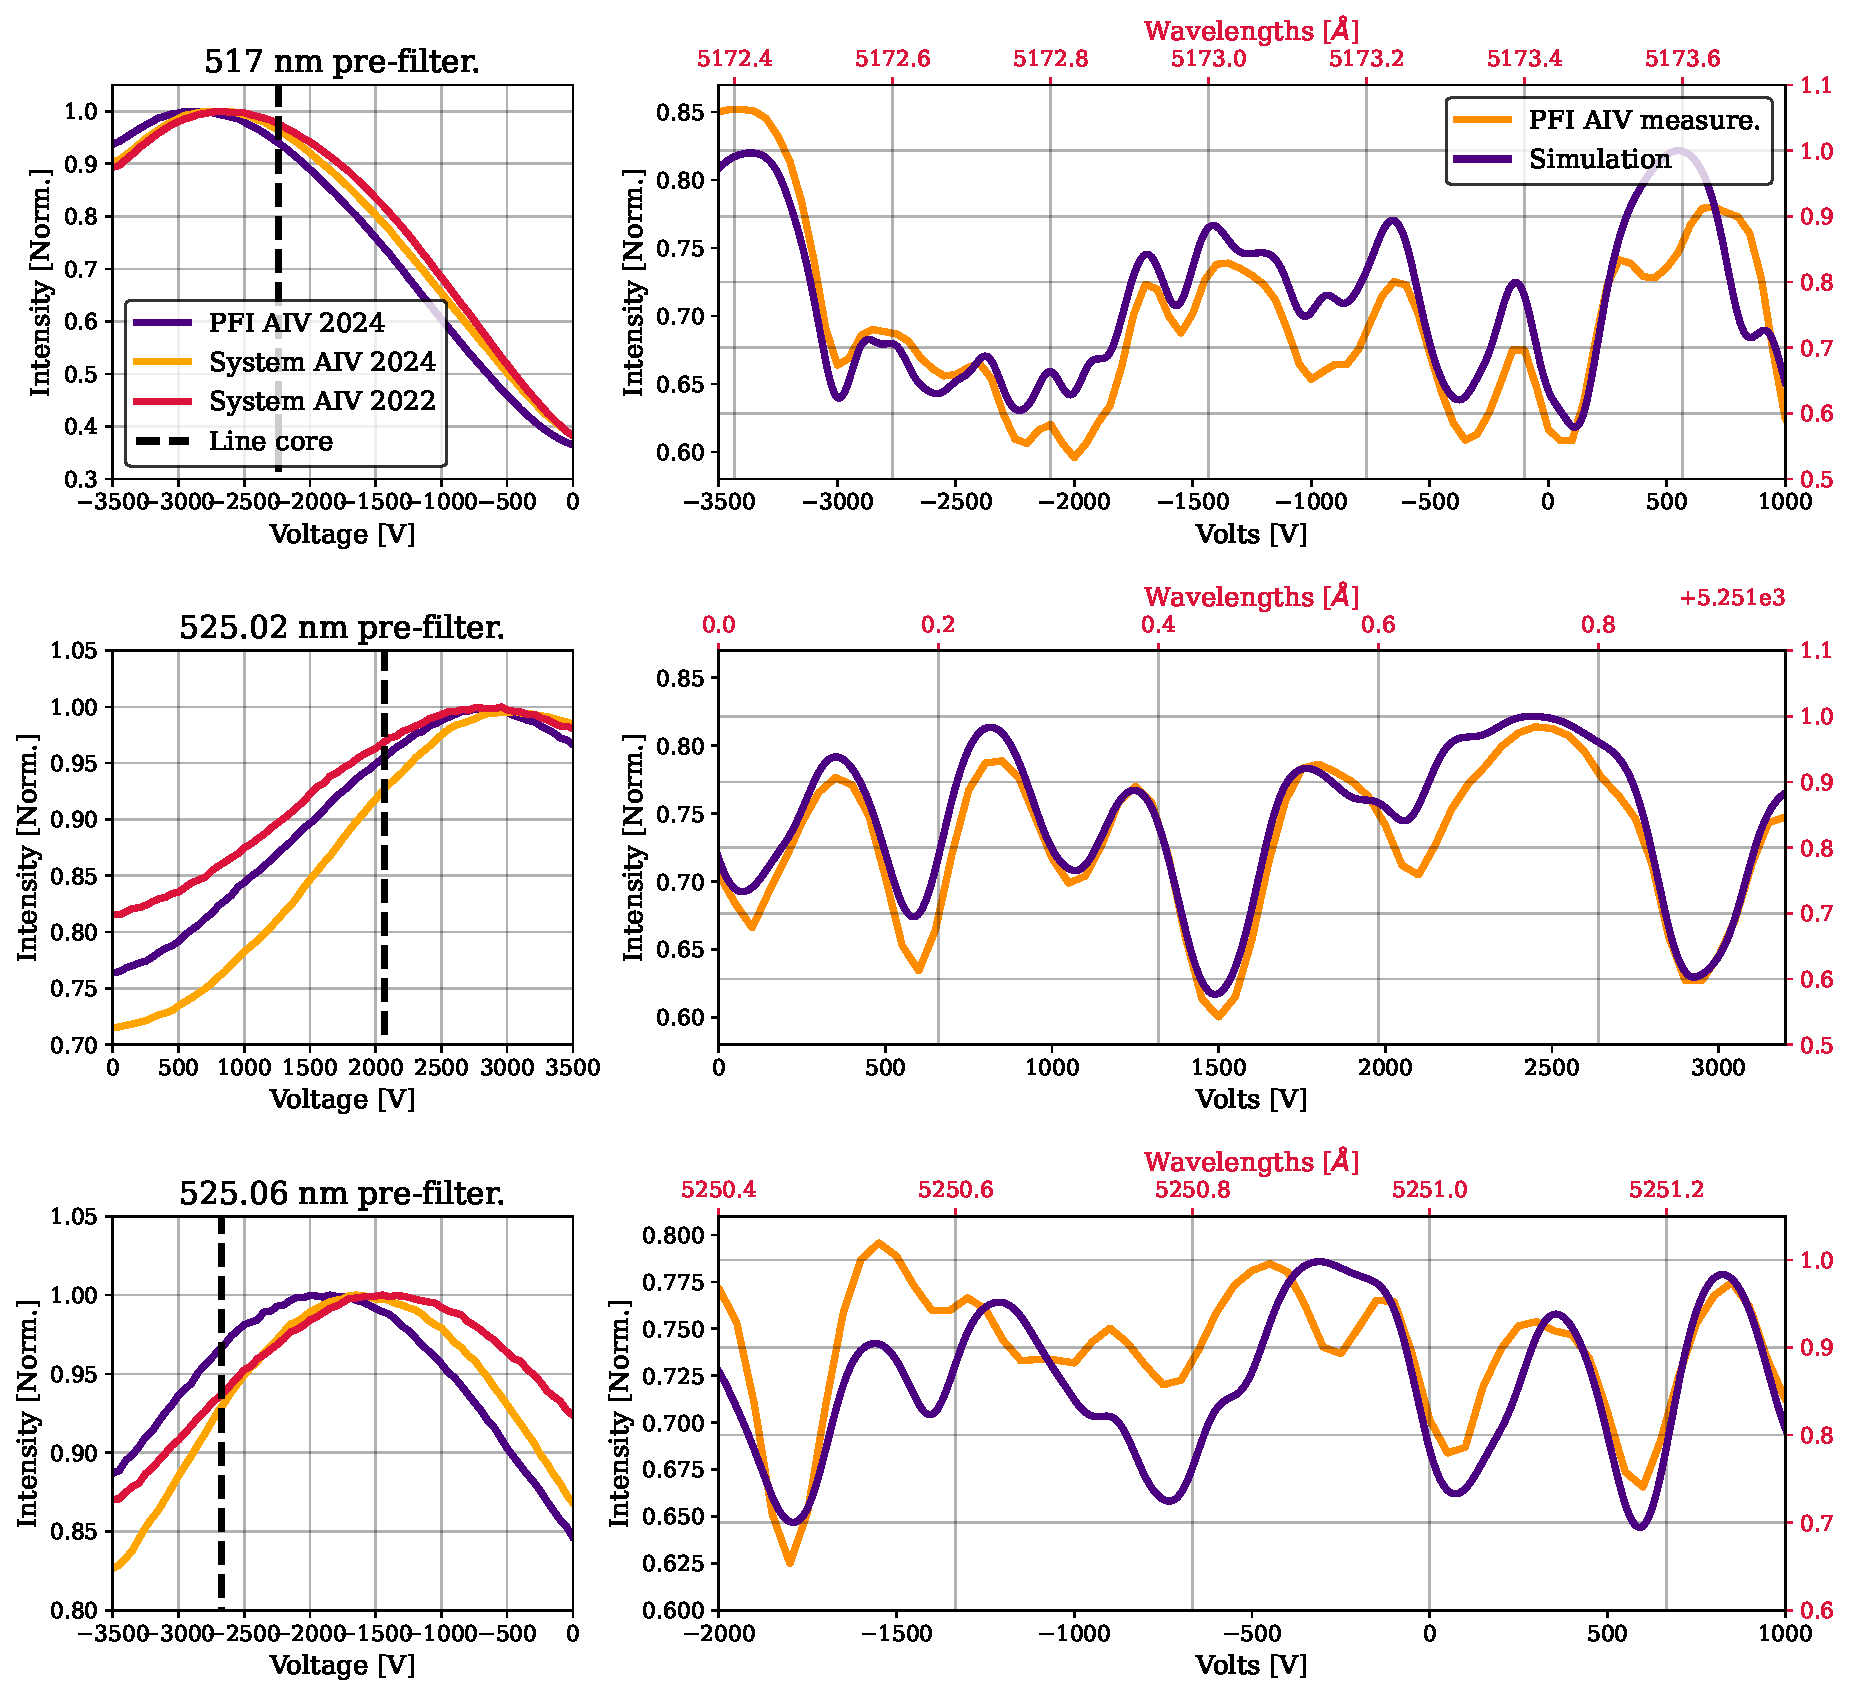
\includegraphics[width=\textwidth]{figures/TuMag/Spectroscopic_calibration.pdf}
    \caption{
      TuMag spectroscopic calibration results. Each row shows results for the 517 nm, 525.02 nm and 525.06 nm pre-filters, from top to row. The left column shows measurements of the pre-filters carried out with a flat LED on different stages of the AIV phases. The right column shows the fit of the I$_2$ cell observation with a simulation employing an etalon with a reflectivity of 0.892 (FWHM$\sim 0.87$). Note that the absolute value of the wavelengths of the simulation (red axis) might be shifted with respect to real values due to unknown conditions of the reference.   
      \label{fig_tumag: spectroscopic_results}}
\end{figure}

TuMag's etalon (see Table \ref{table: Tumags etalon}) operates in a collimated setup with a transmission profile with a FWHM of 0.87 pm (in the double-passs configuration), thus achieving a spectral resolution that exceeds the required 9 pm. Observations of an iodine cell illuminated with a diode were conducted to verify the transmission profile's shape and accurately assess the tuning constant. The right column of Fig.~\ref{fig_tumag: spectroscopic_results} presents, in orange, the iodine cell measurements obtained during the assembly, integration, and verification (AIV) phase of TuMag's integration into the Post Focal Instruments (PFI) platform, which took place at the Max Planck Institute for Solar System Research (MPS) in Göttingen, Germany, in November 2023. Additionally, the dark blue line in the figure represents a simulation of the iodine spectrum observations. This simulation was generated using an analytical model of the transmission profile of collimated etalons (see section \ref{susec_etalon_theory: collimated} for a detailed overview of the model). The results confirm that the spectral resolution achieved in the iodine cell observations is consistent with the estimated 0.87 pm resolution. Furthermore, these observations enabled the calculation of the etalon's tuning constant by identifying corresponding line cores between the simulation and observation and applying a standard least squares fitting to establish the relationship, which was measured in 3300 V/\r{A}.


\begin{figure}
    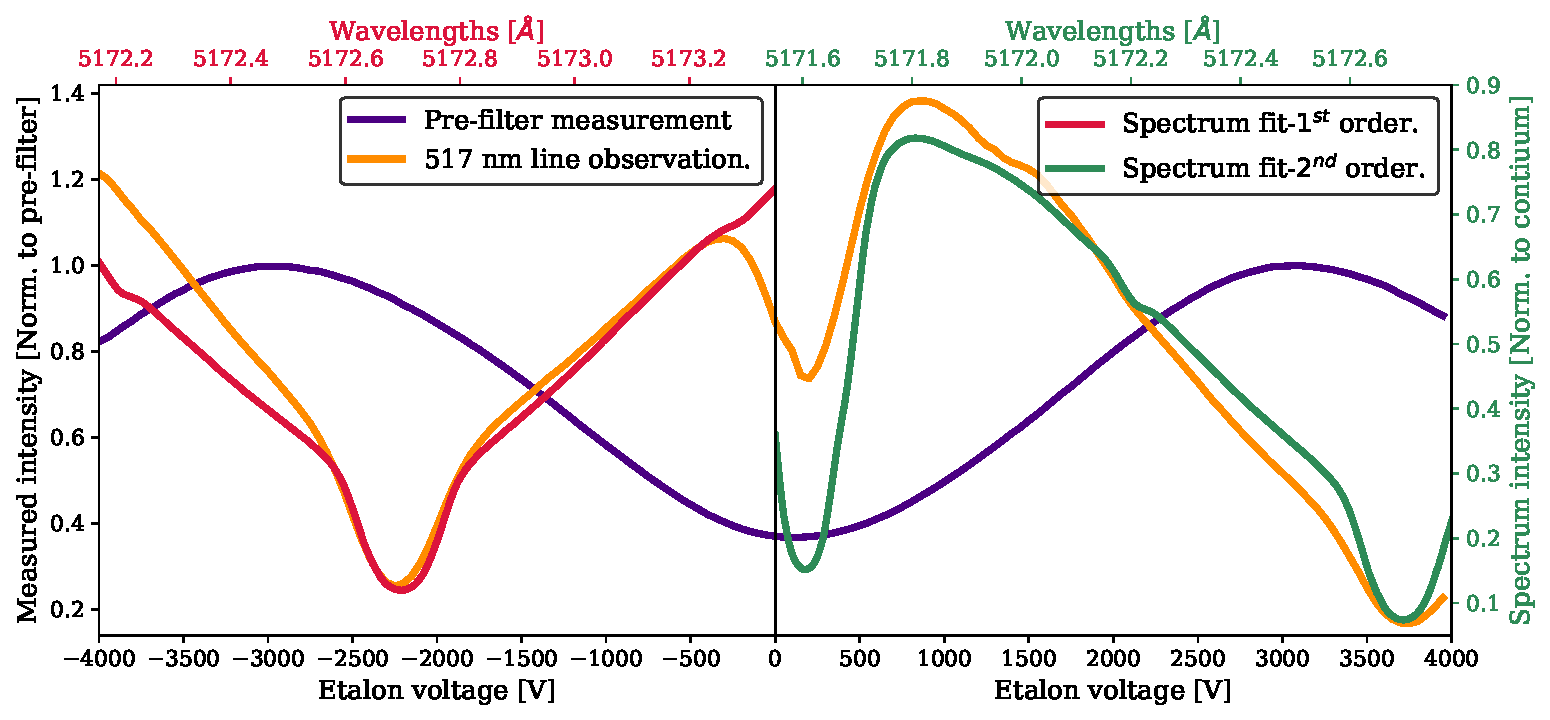
\includegraphics[width=\textwidth]{figures/TuMag/secondorder.pdf}
    \caption{
      Results of the spectroscopic calibration during the end-to-end calbrations of the AIV phase of 2021. The dark blue curve represents the measurement of the 517 nm pre-filter, alongside an observation of the magnesium line using the coelostat at INTA facilities, shown in orange. Two different fits of the solar spectrum are overplotted on the figure. The red line represents a fit to the primary etalon order (negtive voltages), while the green line corresponds to a fit to the second etalon order (positive voltages).      
      \label{fig_tumag:second-order_cont}}
\end{figure}


An observtion of the solar spectrum with the 517 nm pre-filter carried out at INTA facilities on December 2021 during the end-to-end calibration tests is shown in Fig.~\ref{fig_tumag:second-order_cont}, along with the pre-filter mesurement. The magnesium line core is measured at -2200 V aprroximately, with the primary order of the etalon, and can be measured again at approximately 3750 V with a secondary order. A fitting of the solar spectrum \footnote{referencia} is also shown, for both orders. These results reveal substantial contamination from the secondary order near the pre-filter's minimum transmittance. Around 0 volts, the observed spectrum (orange line) combines contributions from both the primary (red line) and secondary (green line) orders. This contamination is particularly significant for data processing because continuum measurements of the magnesium line are generally conducted at -80 V. The contamination predominantly affects the magnesium line, as its broader profile necessitates continuum measurements farther from the line core. In contrast, iron lines, which are narrower, do not require continuum measurements at such significant offsets from the line core.


\subsection{Imaging performance.}
TuMag captures photons using two custom-made cameras \citep{tumag-cams} equipped with GPIXEL back-illuminated GSENSE400BSI detectors, each featuring a $2k \times 2k$ pixel array. These cameras provide a broad FoV of $63'' \times 63''$, sufficient to encompass an entire medium-sized active region, with a plate scale of $0.0378''$/pixel.

In order to fulfill the requirement of the wavefront error of $W \sim \lambda / 14$, the instrument must have means to correct for the additional aberrations introduced by the telescope, the image stabilization and light distribution (ISLiD) system and uncorrected jittering. For this purpose, TuMag is equipped with a PD plate in the filter wheel that allow to apply image reconstruction techniques to the final images. 



